\chapter{人工智能的提示工程}

在人工智能蓬勃发展的当下,提示工程(Prompt Engineering)这一概念应运而生,它如同一把精巧的钥匙,开启了人工智能应用的全新大门,为人们与人工智能之间的交互带来了前所未有的便捷。在本章中,首先对提示工程进行简要介绍;然后详细介绍提示工程的技巧;最后,再介绍与提示工程相关的实际应用。  

\section{提示工程简介}

在本小节中,将引入提示工程这一概念,主要围绕其定义、发展历程以及重要性等方面进行介绍,让读者对提示工程有一个基本的认知。

\subsection{定义与内涵}

提示工程,简而言之,就是针对人工智能模型设计和构建特定的提示(prompt),以引导模型按照预期的方式生成内容、执行任务或做出决策。这里的提示并非简单的指令,而是一种精心构造的文本、图像或其他形式的输入信息,它能够充分挖掘和激发人工智能模型的潜力,使其输出更加精准、更加贴合人类需求的内容。

作为一个新兴的人工智能领域,提示工程涵盖了多个层面。首先,它涉及到对人工智能模型工作原理的深入理解。不同模型的架构、相关的训练数据以及算法机制,决定了模型在处理和输出信息时的侧重点和优势所在。例如,一些基于大规模文本语料训练的自然语言处理模型,擅长理解和生成流畅、连贯的文本内容;而另一些专注于图像识别的模型,则在图像特征提取和分类方面表现出色。只有充分把握模型的特点,才能设计出契合其“思维”方式的提示。

其次,提示工程融合了跨学科的知识与技能。它不仅需要计算机科学、人工智能领域的专业知识,还与语言学、心理学、认知科学等学科紧密相连。在设计提示时,要考虑到人类语言的复杂性、语义的多样性以及人类认知的局限性等因素,从而让提示更加符合人类的表达习惯和理解逻辑,使人工智能模型能够更好地“读懂”人类的意图。

\subsection{发展历程}

提示工程的发展历程与人工智能技术的进步紧密相连,大致可以分为几个阶段。

在早期,人工智能模型相对简单,主要依赖于规则和逻辑进行推理和决策。当时的提示形式较为单一,多为一些简单的指令或查询语句,如“判断这个图形是三角形还是四边形”,“列出符合特定条件的数据记录”等。这些提示主要基于模型预设的规则库,模型按照既定的逻辑路径进行匹配和响应,应用范围相对有限,且对复杂问题的处理能力较弱。

随着机器学习技术的兴起,尤其是深度学习的蓬勃发展,人工智能模型开始具备强大的数据驱动学习能力。这一时期,提示工程逐渐崭露头角。研究人员发现,通过精心设计的提示,可以引导模型更好地挖掘数据中的潜在规律和模式。例如,在自然语言处理领域,通过构造特定的文本提示,模型能够生成具有一定逻辑和语义连贯性的文本段落,如续写故事、生成新闻报道等。在图像处理方面,提示可以帮助模型更准确地识别图像中的物体、场景等元素,并进行相应的分类和标注。

近年来,随着大型语言模型(LLM)和多模态模型的涌现,提示工程迎来了新的发展机遇。这些模型具有海量的参数和丰富的知识储备,能够理解和生成多种模态的信息,如文本、图像、音频等。提示工程在这个阶段变得更加复杂和多样化,不仅需要考虑文本提示的设计,还要兼顾图像、声音等其他模态的提示构建。同时,为了充分发挥大型模型的潜力,研究人员开始探索更加灵活、智能的提示策略,如自适应提示、动态提示生成等,以应对不同场景下复杂多变的任务需求。

\subsection{重要性与价值}

提示工程在人工智能领域具有极其重要的地位和价值,主要体现在以下几个方面。

\paragraph{1. 提升模型性能}

一个精心设计的提示能够显著提升人工智能模型的性能。它可以帮助模型更准确地理解任务要求,减少歧义和误解,从而生成更高质量的输出结果。例如,在文本生成任务中,合适的提示可以引导模型生成更具创意、更符合语境的文本内容;在图像识别任务中,恰当的提示能够提高模型对图像细节的捕捉能力和分类准确性。通过不断优化提示,可以挖掘出模型的潜在性能,使其在各种应用场景中发挥出更好的效果。

\paragraph{2. 拓展应用边界}

提示工程为人工智能的应用拓展了广阔的边界。借助不同的提示,可以将同一模型应用于多种不同的任务和场景,实现一模多用。例如,一个通用的大型语言模型,通过设计不同的文本提示,既可以用于撰写学术论文、创作小说,还可以用于生成商业策划文案、编写代码注释等。这种灵活性大大降低了模型的开发和部署成本,提高了模型的实用性和经济性,使得人工智能技术能够更广泛地渗透到各个行业和领域。

\paragraph{3. 增强人机协作} 

在人机协作的场景中,提示工程起到了至关重要的桥梁作用。它使得人类能够以更加自然、直观的方式与人工智能模型进行交互,将自己的意图和需求清晰地传达给模型。同时,模型也能够根据提示更好地理解人类的指令,做出符合人类期望的响应。这种高效的沟通机制有助于建立起人与机器之间的信任和默契,促进双方在复杂任务中的紧密协作,共同完成更具挑战性的目标,如科学研究、艺术创作、复杂决策支持等。

\paragraph{4. 推动技术创新} 

提示工程的发展不断推动着人工智能技术创新的浪潮。为了设计出更优秀的提示,研究人员需要深入探索模型的内部机制、优化算法、数据处理方法等关键技术。同时,提示工程的应用实践也反过来为模型的改进和完善提供了宝贵的反馈和灵感。例如,通过分析提示在不同模型上的效果差异,可以发现模型在特定方面的不足,从而引导研究人员对模型架构进行调整和优化;在多模态提示的研究过程中,催生了一系列新的数据融合、跨模态学习等技术方法,进一步拓展了人工智能技术的内涵和外延。

综上所述,提示工程作为人工智能领域的一个关键环节,正以其独特的魅力和强大的功能,引领着人工智能技术向着更加智能、高效、实用的方向发展,为人类社会的进步和变革注入源源不断的动力。

\section{提示技巧}

在人工智能提示工程中,掌握有效的提示技巧是提升模型性能和输出质量的关键。以下是一些经过实践验证的提示技巧,这些技巧可以帮助用户更好地与人工智能模型进行交互,实现更精准、高效的任务执行。每种提示方法都配有具体的示例,以便读者更好地理解和应用这些技巧。

\subsection{基于样本数量的提示词技术}

\paragraph{1. 零样本提示(Zero-shot Prompting)} 

零样本提示是一种不依赖于示例数据的提示方式,直接向模型提出问题或任务,让模型依据其内部知识进行回答。这种方法的核心在于模型能够凭借已有的知识体系,在没有外部指导的情况下处理任务。零样本提示通常适用于任务较为简单且模型在特定领域已有足够知识积累的情况。它的优势在于无需提供额外的训练数据或示例,能够迅速处理各种新颖或未见过的任务。通过这种方式,模型的泛化能力和知识推理能力得以充分发挥,尤其在面对一些通用问题时,能够提供及时且准确的答案。

然而,零样本提示的有效性取决于模型的预训练和知识覆盖范围。如果问题涉及到特定领域的专业知识,且模型未曾接触过相关信息,则模型的回答可能会不够准确或缺乏深度。因此,尽管零样本提示具有较高的灵活性,它在面对高度专业化或复杂的任务时可能存在一定的局限性。

假如为了询问“太阳为什么是圆的?”这个问题。这种问题通常属于基础天文学范畴,模型可以根据其已知的物理学原理来回答,例如通过引力均匀地吸引周围物质,使得太阳在自转过程中呈现出近似的圆形结构。

\begin{lstlisting}[language={python},label={},caption={}, basicstyle=\footnotesize\ttfamily, breaklines=true, numbers=left, frame=single]
prompt :太阳为什么是圆的?  
\end{lstlisting}

再如,让人工智能“解释一下量子纠缠现象。”,量子纠缠是量子力学中的一种现象,模型可以直接利用其物理学领域的知识来解释量子纠缠的基本概念和影响,例如两粒子间即使相隔很远,依然能即时互相影响的性质。

\begin{lstlisting}[language={python},label={},caption={}, basicstyle=\footnotesize\ttfamily, breaklines=true, numbers=left, frame=single]
prompt :解释一下量子纠缠现象。  
\end{lstlisting}

这些例子展示了零样本提示如何通过简单的提问,让模型基于其知识库快速生成准确的答案。

\paragraph{2. 少样本提示(Few-shot Prompting)} 

少样本提示是一种通过提供少量示例来帮助模型理解任务要求的方法。这种技术在面对任务复杂性较高,或模型需要掌握特定任务格式时尤为有效。与零样本提示不同,少样本提示通过展示几个具有代表性的示例,让模型能够从这些示例中学习任务的模式和结构,然后将这种学习转化为对类似任务的处理能力。通过这种方式,模型能够快速掌握并应用任务的具体要求,避免了直接进行全新任务的困难。

少样本提示的关键在于示例的选择。所提供的示例需要具有代表性,能够准确地展示任务的特点和要求。例如,在数学问题的加法任务中,给出几个简单的示例可以帮助模型理解数字加法的规则;在文本摘要任务中,展示一些简洁而准确的摘要示例,可以引导模型生成高质量的摘要。通过这种方式,模型在完成实际任务时会更加高效和准确。

少样本提示不仅提高了任务的处理效率,而且大大降低了对大量训练数据的依赖,特别适用于那些数据量有限或时间紧迫的应用场景。不过,少样本提示的效果仍然取决于示例的质量和代表性,如果示例不够精准或多样,模型可能无法充分理解任务的精髓,进而影响结果的准确性。

例如,在数学加法的任务中,以下提供几个简单的加法示例,可以帮助模型理解加法运算的规则。通过这种提示方式,模型能够迅速掌握任务,并对类似的问题作出正确回答。

\begin{lstlisting}[language={python},label={},caption={}, basicstyle=\footnotesize\ttfamily, breaklines=true, numbers=left, frame=single]
示例1:
问题:2 + 3 =
答案:5

示例2:
问题:7 + 8 =
答案:15

现在,请解答以下问题:
问题:15 + 27 =
答案:
\end{lstlisting}

在文本生成摘要任务中,提供少量的原文和摘要示例,可以帮助模型理解如何提取关键点并用简洁的语言呈现要点。这对于需要生成简明扼要总结的任务尤为重要。

\begin{lstlisting}[language={python},label={},caption={}, basicstyle=\footnotesize\ttfamily, breaklines=true, numbers=left, frame=single]
示例1:
原文:人工智能是计算机科学的一个分支,致力于创造能够模拟人类智能的系统。
摘要:人工智能旨在模拟人类智能。

示例2:
原文:气候变化导致了全球气温上升,极端天气事件频发。
摘要:气候变化引发全球变暖和极端天气。

现在,请为以下文本生成摘要:
原文:大数据技术的发展使得数据分析更加高效和精准。
摘要:
\end{lstlisting}

通过少样本提示,模型能够通过从少量示例中推断出任务的核心特征,并快速应用这些知识来生成正确的结果。这种方法不仅节省了训练时间,还提高了处理复杂任务的效率。

\subsection{基于思考过程的提示词技术}

\paragraph{1. 链式思考提示(Chain-of-Thought Prompting)} 

链式思考提示是一种引导模型在给出最终答案之前,先分步骤展示思考过程的技术。这种方法不仅有助于提升模型的推理能力,而且能够增强答案的透明度,让用户理解模型是如何得出结论的。通过将思考过程明确拆解,链式思考提示使得模型能够更有条理地处理复杂问题,并在每个步骤中逐步验证自己的推理。这种方式的优势在于,它减少了推理过程中的不确定性,使得最终的答案更具可信度。

链式思考提示尤其适用于解决需要多步推理的任务,如数学问题、逻辑推理和复杂决策分析。在这些任务中,直接给出答案往往缺乏解释,而通过分步骤推理,模型可以逐步清晰地展示其解决问题的思路和方法。这不仅有助于提高答案的准确性,也能帮助用户更好地理解解决问题的过程,进而提升与模型的互动效果。

这种方法的实施需要一定的策略,模型需要能够在推理过程中保持逻辑的连贯性,并确保每一步的推导都是基于正确的前提条件。链式思考提示的一个潜在挑战是,过于复杂或不明确的提示可能导致模型在某个步骤出错,从而影响最终结果的正确性。因此,合理地引导模型逐步推理是确保链式思考提示成功的关键。

例如,在解决数学问题过程中,链式思考提示通过将问题拆解为多个步骤,引导模型逐步完成计算,从而得出正确的答案。特别是在几何或代数题目中,分步骤的推理过程能够帮助模型避免直接跳跃到结论,确保每个步骤的推导都是合理且准确的。

\begin{lstlisting}[language={python},label={},caption={}, basicstyle=\footnotesize\ttfamily, breaklines=true, numbers=left, frame=single]
题目:如果一个三角形的两边分别为3和4,且夹角为90度,求第三边的长度。

解题步骤:
1. 根据勾股定理,第三边的平方等于3的平方加4的平方。
2. 计算3² + 4² = 9 + 16 = 25。
3. 第三边的长度是√25 = 5。
答案:5
\end{lstlisting}

再如,在图像生成方面,如果想要生成一幅冬季山景画,可以按如下提示进行。

\begin{lstlisting}[language={python},label={},caption={}, basicstyle=\footnotesize\ttfamily, breaklines=true, numbers=left, frame=single]
题目:生成一幅冬季山景画。

构思步骤:
1. 确定主要元素:雪覆盖的山峰、松树、静谧的湖面。
2. 选择色彩方案:冷色调为主,白色、蓝色和灰色。
3. 构图安排:山峰位于画面中央,湖面在前景,松树分布在两侧。
4. 添加细节:天空中飘落的雪花,湖面反射的山影。
5. 完善光影效果:夕阳的余晖照亮山峰,湖面呈现金属光泽。
答案:
\end{lstlisting}

通过这种分步骤的提示,模型可以确保每一步推理都有据可依,从而提高解题过程的透明度和结果的可靠性。这不仅能帮助模型更准确地得出答案,还能让用户清楚地看到每个推理步骤的逻辑。

\paragraph{2. 自动链式思考提示(Automatic Chain-of-Thought Prompting)} 

自动链式思考提示是在链式思考提示的基础上,通过自动化生成思考步骤的方式,进一步提升模型的推理能力。这种方法的关键在于通过系统化的过程将复杂问题分解成一系列逻辑步骤,帮助模型在没有人工干预的情况下,自动生成思考过程并进行推理。与传统的链式思考提示不同,自动链式思考提示能够在没有明确给定每一步的情况下,通过预设的框架自动推理,极大地提高了处理复杂任务的效率。

这种方法特别适用于那些需要复杂推理的任务,如市场趋势分析、科学研究问题、决策分析等。在这些任务中,涉及多个因素和变量,且每个因素之间存在复杂的相互关系。自动链式思考提示能够帮助模型梳理出这些因素,并通过系统的推理步骤逐一考虑,确保所有关键因素都被纳入考量。这不仅提升了推理的准确性,还使得整个思考过程更加高效,避免了人工干预的复杂性。

自动链式思考提示的优势在于其高效性和一致性。通过自动化推理过程,模型可以在面对类似任务时,快速生成思考步骤,减少重复性的工作,并且能够在短时间内对多个任务进行高效处理。不过,自动化的过程也存在一定的风险,如果推理框架或步骤设计不当,可能导致推理路径不合理,进而影响最终的结果。因此,在实际应用中,合理设计自动化推理框架是确保这种方法成功的关键。

例如,在市场趋势分析的任务中,自动链式思考提示通过系统化的步骤来引导模型逐一分析各个关键因素,并结合数据和趋势进行预测。这个过程涉及到多个变量的综合考虑,因此自动化推理能够显著提高任务执行的效率和准确性。

\begin{lstlisting}[language={python},label={},caption={}, basicstyle=\footnotesize\ttfamily, breaklines=true, numbers=left, frame=single]
题目:分析当前智能手机市场的趋势,并预测未来的发展方向。

解题步骤:
1. 收集最近一年的智能手机销售数据。
2. 分析不同品牌的市场份额变化。
3. 研究消费者偏好的变化,如对5G、摄像头性能的需求。
4. 考虑技术创新对市场的影响,如折叠屏、人工智能功能。
5. 综合以上因素,预测未来智能手机市场的发展方向。
答案:
\end{lstlisting}

通过这种自动化的思考过程,模型能够自如地处理复杂的市场分析任务,不仅节省了大量人工时间,还能确保在分析中涵盖所有关键因素,提供更全面且具有预测价值的结论。

\paragraph{3. 逻辑链式思考提示(Logical Chain-of-Thought Prompting)} 

逻辑链式思考提示是一种强调逻辑严密性的方法,旨在引导模型在思考过程中遵循严格的逻辑顺序,以减少推理中的错误和不准确性。这种方法特别适用于需要严谨逻辑推理的任务,尤其是涉及复杂因果关系、科学原理或法律推理等领域。通过确保每一步推理都有明确的依据并紧密衔接,逻辑链式思考提示能够有效减少模型输出中的逻辑错误和幻觉,从而提高最终答案的可靠性和准确性。

逻辑链式思考提示不仅要求模型清晰地理解每一步推理的内在逻辑,还需要确保推理的每个环节都能够与前后的步骤保持一致性。在面对复杂问题时,合理的逻辑结构能够帮助模型从多个维度、多个步骤逐步推导出正确的结论,避免跳跃式推理或未经验证的假设。与其他类型的思考提示相比,逻辑链式思考提示的优势在于它通过系统化的逻辑分析,确保模型能够逐步消除潜在的推理偏差和误解。

在实际应用中,逻辑链式思考提示常常应用于那些具有强烈因果关系的任务,如科学实验分析、推理问题和决策支持等。通过分步骤分析每个环节,模型不仅能够得出一个合理的结论,还能让用户清晰地看到每一步推理的依据。这种透明度对于提高用户对模型结果的信任度具有重要作用。

例如,在分析科学实验的任务中,逻辑链式思考提示能够帮助模型按照实验的因果关系逐步推理,确保每个环节的推导过程清晰、严谨。例如,在分析光合作用过程中,模型需要按照光能转化为化学能的科学原理逐步推理,并确保每一步的解释都有坚实的科学依据。



\begin{lstlisting}[language={python},label={},caption={}, basicstyle=\footnotesize\ttfamily, breaklines=true, numbers=left, frame=single]
题目:分析光合作用过程中光能转化为化学能的逻辑步骤。

解题步骤:
1. 光能被叶绿体中的叶绿素吸收。
2. 吸收的光能用于水分子的分解,释放氧气和电子。
3. 电子通过电子传递链释放能量,生成ATP和NADPH。
4. ATP和NADPH用于二氧化碳的固定,生成葡萄糖。
5. 最终,光能转化为储存在葡萄糖中的化学能。
答案:
\end{lstlisting}

通过这种精确且符合逻辑的步骤,模型能够清楚地展示光合作用的每个环节如何相互作用,并最终导致光能转化为化学能。这种方法不仅提高了答案的准确性,还能让用户更加信服模型所提供的推理过程,因为每一步都有清晰的科学依据和逻辑支持。

\paragraph{4. 符号链提示(Chain-of-Symbol Prompting)} 

符号链提示是一种利用符号代替自然语言构建提示的技术,旨在帮助模型更好地处理涉及复杂空间关系的任务,尤其是在数学、物理或其他需要精准计算和空间推理的领域。这种方法通过符号化的表示,使得模型能够在符号的框架内进行更为高效和精确的推理,避免了自然语言表达中的歧义和不确定性。符号链提示尤其适用于涉及数学公式、几何图形、物理公式等任务,因为符号能够清晰地表达量与量之间的关系,且不容易产生理解偏差。

与传统的自然语言提示相比,符号链提示的优势在于它简洁且直观,能够精确描述任务中的关键关系,并且能够帮助模型集中精力解决具体的空间推理问题。在处理复杂问题时,符号提供了一种简洁有效的方式来表达任务的各个方面,避免了过多的文字描述,使得推理过程更加清晰、可控。这种方法尤其在涉及到定量分析和空间计算的任务中展现了强大的能力,因为符号本身具有较强的精确性和数学表达能力。

例如,在几何学和代数中,符号链提示可以用来简化数学题目的表达,使得模型能够更加专注于运用公式和定理来解决问题。在这类任务中,符号化的表达方式不仅能够提高计算效率,还能减少计算过程中的复杂性,帮助模型快速地从已知条件推导出答案。因此,这种方法在数学推理、几何问题、物理实验等任务中具有重要应用价值。

在解决几何问题时,符号链提示能够通过简洁的符号表达清晰地描述各个几何关系,使得模型可以通过符号运算快速得出解答。在此任务中,涉及到勾股定理的应用,符号链提示通过使用公式帮助模型直接进入计算阶段,避免了不必要的语言解释。



\begin{lstlisting}[language={python},label={},caption={}, basicstyle=\footnotesize\ttfamily, breaklines=true, numbers=left, frame=single]
题目:在一个直角三角形中,已知两条直角边分别为a和b,求斜边c的长度。

解题步骤:
1. 使用勾股定理:c² = a² + b²
2. 代入已知值:c² = a² + b²
3. 计算c = √(a² + b²)
答案:c = √(a² + b²)
\end{lstlisting}

通过符号链提示,模型能够专注于数学公式的运用,从而提高空间推理能力并迅速得出准确答案。这种方法使得问题的求解过程更加简洁、直接,同时减少了对复杂语言结构的依赖,极大地提升了计算效率。

\paragraph{5. 思维树提示(Tree-of-Thoughts Prompting)} 

思维树提示是一种将思考过程构建为树状结构的技术,它帮助模型从根节点出发,逐步扩展多个子节点,以探索各种可能的思考路径,并最终找到最佳的解决方案。这种方法特别适用于复杂问题的分析和决策过程,因为它能够系统地梳理出所有可能的步骤和选项,并在每个节点处评估不同的选择。思维树提示使得任务的解决过程更具结构性,不仅能够帮助模型进行全面的思考,还能确保各个环节的考虑不遗漏关键因素。

在思维树结构中,根节点通常表示问题的起点或核心目标,而每个子节点则代表了进一步展开的思考方向。随着树的扩展,思维的层次逐渐加深,模型能够对问题进行多角度、多层次的探索,最终在各个分支中评估不同选择的优劣,找到最优的解决路径。这种方法有助于理清思路,避免过于单一或片面的思考,提升决策的全面性和深度。

思维树提示常常被应用于项目管理、策略规划、问题解决等领域。在这些领域,任务的完成往往涉及多个步骤和决策点,因此,通过构建一个清晰的思维树结构,可以确保每个步骤都得到充分的考虑和讨论,最终形成一个合理且高效的行动计划。

例如,在制定项目计划的过程中,思维树提示可以帮助模型逐步展开每个阶段的任务,并根据不同的需求和条件探索多个实施方案。在这个过程中,每个阶段和任务都有明确的子节点,确保每个环节都得到了详细的规划。通过思维树结构,模型能够全面考虑项目的每个环节,并确保各项任务的协调与执行。



\begin{lstlisting}[language={python},label={},caption={}, basicstyle=\footnotesize\ttfamily, breaklines=true, numbers=left, frame=single]
题目:制定一个为期六个月的软件开发项目计划。

思维树:
1. 项目启动
   - 确定项目目标
   - 分配团队成员
2. 需求分析
   - 收集用户需求
   - 编写需求文档
3. 设计阶段
   - 系统架构设计
   - 界面设计
4. 开发阶段
   - 前端开发
   - 后端开发
5. 测试阶段
   - 功能测试
   - 用户验收测试
6. 部署与维护
   - 部署到生产环境
   - 持续维护与更新
答案:
\end{lstlisting}

在这个示例中,思维树从项目启动开始,逐步展开每个阶段的关键任务和子任务,确保在每个阶段中都涵盖了所有重要的考虑因素。这种结构化的方式不仅帮助模型理清项目的整体规划,还能够对每个环节的执行过程进行细致的安排,以确保项目能够按照既定目标顺利推进。

\paragraph{6. 思维图提示(Graph-of-Thought Prompting)} 

思维图提示是一种通过图形化方式组织思考过程的技术。在思维图中,节点表示各个思考内容或概念,而边则表示节点之间的关系。这种结构化的方法能够帮助模型全面地考虑问题的各个方面,确保在解决复杂问题时,不遗漏任何可能影响结果的因素。与传统的线性思考方式不同,思维图提示能够通过多维度的视角,展示问题的多层次结构和相互联系,从而促进更全面、更深入的分析和推理。

思维图的核心优势在于其图形化和可视化的特点,使得思考过程变得更加直观和清晰。通过将相关的概念、信息或步骤以图形的形式连接,模型能够快速识别出不同节点之间的关联关系,从而在解决问题时避免遗漏重要信息或产生逻辑漏洞。此外,思维图可以帮助模型更好地组织思考过程,将复杂问题分解为多个较小的、可管理的部分,逐步进行分析和推理,最终得出更精确的结论。

思维图提示常用于复杂的分析任务,特别是那些涉及多个因素和维度的场景,如企业战略分析、市场研究、产品开发等。在这些任务中,思维图可以帮助模型系统性地梳理出所有可能的变量和关系,确保每个因素都得到充分的考虑和分析。通过思维图,模型不仅能从整体上把握问题的全貌,还能深入探索各个子问题的具体细节,进而形成更全面的解决方案。

例如,在分析企业的竞争优势时,思维图提示能够帮助模型全面梳理企业在技术、资源、市场等方面的核心能力及其相互关系。通过思维图,模型可以将企业的竞争优势从多个维度展开,明确每个维度所涉及的关键因素,以及这些因素如何共同作用,提升企业的市场竞争力。在此过程中,模型能够通过对每个节点及其连接关系的详细分析,识别出企业的优势和短板,从而制定出有效的战略决策。



\begin{lstlisting}[language={python},label={},caption={}, basicstyle=\footnotesize\ttfamily, breaklines=true, numbers=left, frame=single]
题目:分析一家科技公司的竞争优势。

思维图:
- 核心能力
  - 技术研发
  - 创新文化
- 资源
  - 人才储备
  - 财务状况
- 市场定位
  - 目标客户
  - 品牌影响力
- 运营效率
  - 供应链管理
  - 产品交付速度
- 客户关系
  - 客户服务
  - 用户反馈机制
答案:
\end{lstlisting}

通过这种图形化的提示,模型能够在各个层面上对企业的竞争优势进行全面评估。每个维度的核心因素和相关子因素被清晰地展现,并且通过节点之间的连接,模型可以直观地看到它们之间的相互影响。这不仅有助于提高分析的精确性,还能帮助模型快速识别出可能的改善领域,为企业的战略制定提供有价值的参考。

\subsection{基于一致性和连贯性的提示词技术}

\paragraph{1. 自我一致性(Self-Consistency)} 

自我一致性是一种提示技术,旨在通过让模型对同一问题生成多个答案,然后对这些答案的一致性进行评估,最终选出最一致的答案作为最终输出。该方法能够显著提高答案的可靠性和稳定性,尤其是在处理复杂问题或模型不确定性较高的情况下。通过生成多个答案,模型可以从多个角度或思路进行思考,进而避免因单一推理路径带来的偏差或错误,从而保证输出的答案更加准确且具有更强的可信度。

在许多情况下,模型可能会根据不同的推理路径或已知信息给出多个不同的答案。通过对这些答案进行比较和综合,能够更加全面地揭示问题的真相,减少可能的误导。例如,在科学、技术或复杂的理论问题中,由于模型可能存在信息不完整或理解误差,通过自我一致性方法可以帮助确认哪些答案是合理的,并且从中提炼出最符合问题要求的解释。

自我一致性的核心优势在于它能够增强模型的推理能力,尤其是在面对多样化或模糊性较大的任务时。模型不仅仅提供一个单一的答案,而是通过多次尝试来确保输出的准确性。尤其是在处理一些科学或技术性较强的任务时,模型会受到信息多样性和复杂性的挑战,而自我一致性能够通过这种“多重尝试”的方式,逐步缩小错误的可能性,提供更为准确和可靠的结果。

例如,在解释某些科学概念时,模型可能会根据不同的角度或知识来源产生多个答案。通过应用自我一致性技术,模型能够对这些不同的答案进行比对,筛选出最一致的解释,从而提供更加全面和准确的答案。在这个过程中,每个答案都可能从不同的切入点进行阐述,而最终的综合回答则能够体现出更强的可靠性。



\begin{lstlisting}[language={python},label={},caption={}, basicstyle=\footnotesize\ttfamily, breaklines=true, numbers=left, frame=single]
题目:什么是黑洞?

答案1:
黑洞是宇宙中一种具有极强引力的天体,连光线也无法逃脱。

答案2:
黑洞是由大量物质坍缩形成的天体,具有强大的引力场。

答案3:
黑洞是时空的极端扭曲区域,因其引力作用使得任何物质都无法逃脱。

综合以上答案,黑洞是一种由大量物质坍缩形成的天体,具有极强的引力,甚至连光线也无法逃脱,从而在时空中形成极端扭曲的区域。
\end{lstlisting}

在这个示例中,模型通过生成三个不同的答案,分别从黑洞的引力、物质坍缩和时空扭曲等角度来进行描述。然后,模型对这些答案进行比对和融合,综合出一个更全面且一致的解释。这种方法不仅提高了答案的准确性,也使得模型能够给出更加严谨、符合科学原理的答案。因此,自我一致性方法能够在处理诸如科学解释、复杂理论等任务时,大大提升模型的推理能力和结果的可靠性。

如果需要生成一幅黑洞的科幻艺术图,可以按照如下提示进行。



\begin{lstlisting}[language={python},label={},caption={}, basicstyle=\footnotesize\ttfamily, breaklines=true, numbers=left, frame=single]
题目:生成一幅黑洞的科幻艺术图。

答案1:
黑洞位于画面中央,周围有旋转的光环,吸引着周围的星际物质,背景是深邃的宇宙星空。

答案2:
一个巨大的黑洞吞噬着周围的星球,光芒四射的喷流从黑洞两侧喷出,背景是绚丽的星云。

答案3:
黑洞的强大引力场扭曲了周围的时空,形成独特的光环效果,周围散布着耀眼的星辰和行星残骸。

综合以上答案,黑洞位于画面中央,其强大的引力场扭曲了周围的时空,形成旋转的光环,吸引并吞噬着周围的星际物质。两侧喷出的耀眼喷流与背景中绚丽的星云和深邃的宇宙星空相映成趣,营造出壮观而神秘的科幻艺术效果。
\end{lstlisting}

在这个示例中,模型通过生成三个不同版本的黑洞科幻艺术图描述,然后综合这些描述,得出一个更全面且一致的视觉效果。这种方法不仅提高了图像生成的准确性,也使得模型能够给出更加严谨、符合科学原理和艺术美感的图像描述。因此,自我一致性方法能够在处理诸如科幻艺术创作、复杂场景描绘等任务时,大大提升模型的创作能力和结果的可靠性。

\paragraph{2. 对比链式思考提示(Contrastive Chain-of-Thought Prompting)} 

对比链式思考提示通过引导模型对比不同的思考路径或答案,帮助模型识别和理解其中的差异,从而提高其对问题的全面理解和推理能力。这种方法在处理需要多角度分析和权衡不同方案的任务时尤其有效。通过对比,模型不仅能更好地掌握不同选项之间的优缺点,还能在此基础上做出更具逻辑性和一致性的决策。

与传统的单一路径思考不同,对比链式思考提示鼓励模型同时考虑多个解决方案,并评估每个方案的效果。通过这种方式,模型可以逐步理清每个选项的利与弊,找出最适合特定情境的解决方案。这种思维方式不仅增加了答案的可靠性,还增强了答案的连贯性和一致性,避免了单一视角带来的片面性。

在实际应用中,这种方法广泛适用于决策、规划等任务,特别是在需要权衡多种不同因素时,例如市场策略、资源分配、产品设计等。通过对比分析不同方案的特点和预期效果,模型可以帮助用户更清晰地理解每个选择的潜在影响,从而做出更加明智和科学的决策。

例如,在市场营销策略选择的任务中,模型需要对比不同的营销方式,根据目标受众、预算、传播途径等因素,评估每种策略的优缺点。通过对比,模型能够帮助决策者更清晰地理解每个策略的优势和适用场景,从而做出最佳选择。



\begin{lstlisting}[language={python},label={},caption={}, basicstyle=\footnotesize\ttfamily, breaklines=true, numbers=left, frame=single]
题目:为新产品选择最佳的市场营销策略。

策略A:
1. 通过社交媒体广告增加品牌曝光。
2. 举办线上促销活动吸引消费者。
3. 利用网红合作推广产品。

策略B:
1. 进行电视和广播广告宣传。
2. 在实体店铺设置展示区。
3. 发送电子邮件营销给潜在客户。

对比分析:
- 策略A更适合年轻受众,具有较高的互动性和传播速度。社交媒体广告能够迅速吸引年轻人群体的关注,线上促销活动则具有较低的成本和较高的灵活性,能够快速反馈效果。而网红合作能够提升品牌的可信度和传播效果,尤其是在短视频平台中表现尤为突出。
- 策略B则覆盖面较广,适合那些目标受众群体较为广泛的情况,但成本相对较高,尤其是电视和广播广告的投入较为昂贵。此外,尽管实体店展示和电子邮件营销能够为线下客户提供更直观的体验,但互动性相对较弱,且传播速度较慢。

最佳策略的选择应根据目标受众和预算情况来决定。若目标群体主要为年轻人且预算有限,策略A将是更为合适的选择;而如果目标是覆盖更广泛的受众,且预算充足,策略B则更具优势。
\end{lstlisting}

在这个示例中,通过对比两种不同的市场营销策略,模型清晰地展示了每个策略的特点、适用场景及其优缺点。通过这种对比分析,模型不仅帮助决策者更好地理解每种策略的优势,还能提供更为深刻的决策依据。

\subsection{基于知识和信息的提示词技术}

\paragraph{1. 生成知识提示(Generated Knowledge Prompting)} 

生成知识提示是一种通过引导模型先生成与任务相关的知识,再利用这些生成的知识来完成任务的技巧。这种方法的核心在于先让模型自我提取并总结出相关背景信息,从而使模型在处理复杂问题时,能够获得更全面的视角,避免因知识不足或背景信息缺乏而导致的错误判断或遗漏。在面对需要广泛背景知识支撑的问题时,生成知识提示尤其有效,它能帮助模型在没有明确指令的情况下,主动收集和整合有用信息,为后续分析和决策提供扎实的基础。

这一技巧的实施通常分为两个步骤。第一步是生成相关的背景知识,通常通过模型从已有的知识库中提取并生成信息。第二步是在这些知识的基础上进行任务分析,结合具体问题进行推理,得出最终的解决方案。这种方法不仅能提高模型的理解深度,还能够在多维度上分析问题,从而提升结果的准确性和可靠性。

生成知识提示对于处理那些需要全面、深入理解的任务具有重要作用,尤其是在分析性任务中,可以有效帮助模型跳出常规的思维框架,结合更加广泛的视角进行问题的全面分析。通过这种方式,模型能够更好地理解复杂问题的多层次背景,为解决问题提供更加系统化的思路。

例如,在分析气候变化对生态系统的影响时,模型需要理解气候变化的各方面效应,并将这些影响综合考虑。通过生成相关的背景知识,模型能够自如地将不同领域的信息整合在一起,提供更加全面的分析结果。



\begin{lstlisting}[language={python},label={},caption={}, basicstyle=\footnotesize\ttfamily, breaklines=true, numbers=left, frame=single]
题目:分析气候变化对全球生态系统的影响。

第一步,生成相关知识:
- 气候变化导致全球气温上升,极端天气事件更加频繁。
- 极端天气事件如飓风、洪水和干旱,对生态系统的破坏加剧。
- 海平面上升威胁沿海生态系统,导致栖息地丧失。
- 生物多样性受到威胁,部分物种面临灭绝风险。

第二步,利用这些知识进行分析:
气候变化通过多种途径影响全球生态系统。首先,全球气温上升直接导致冰川融化,进而导致海平面上升,威胁到沿海地区的生态环境。其次,随着极端天气事件的增加,如飓风、洪水、干旱等,这些自然灾害不断破坏动植物的栖息地,迫使许多物种迁移或面临灭绝的风险。此外,气候变化还加剧了生物多样性的减少,许多物种在气候变化的压力下无法适应新环境,导致生态平衡的进一步失衡。温度的升高以及栖息地的减少使得生态系统中的物种迁移受到限制,生态功能也遭到破坏。这些变化不仅对自然环境造成严重威胁,也影响到人类社会的各个方面,如农业生产、经济发展以及人类健康等。
\end{lstlisting}

通过这种生成知识提示,模型能够从多个维度出发,全面分析气候变化对生态系统的影响。生成的背景知识为模型提供了深入理解问题所需的所有关键信息,进而使其能够进行更加复杂的推理,得出具有高准确性的分析结论。

\paragraph{2. 知识链提示(Chain-of-Knowledge Prompting)} 

知识链提示是一种通过引导模型按照逻辑顺序逐步构建知识框架的方式,旨在帮助模型在解决问题时逐步积累和整合关键信息,以生成更加准确和深刻的答案。这种方法强调在思考和推理过程中,遵循一定的知识体系,确保每个步骤都是基于前一步骤的合理推导,进而提高模型的理解能力和推理质量。通过知识链提示,模型能够有条不紊地处理复杂的问题,从多个维度和角度对问题进行深入分析。

这种提示方式尤其适用于那些涉及多个因素或维度的问题,它帮助模型在面对复杂的因果关系、历史事件、社会现象等任务时,有效理清各个因素之间的联系,并逐步深入探讨每个因素的作用。与零样本提示和少样本提示不同,知识链提示不单纯依赖于模型已有的知识,而是通过逻辑推理和步骤化思考,带领模型构建起系统的知识框架,确保其推理过程更加完整和可靠。

通过这种方式,模型不仅能够在任务执行中保持较高的连贯性,还能够逐步提升对问题的综合理解,避免单一视角下的偏见或遗漏,使得生成的答案更加全面且有深度。知识链提示的核心优势在于它能够引导模型系统性地思考,逐层揭示问题背后的因果关系和内在逻辑,特别适合于涉及历史分析、复杂决策或多因素分析的任务。

例如,在分析工业革命的背景时,通过知识链提示可以帮助模型系统地了解并阐释多个因素如何交织在一起,推动了这一历史性变革的发生。每个因素的作用都被逐一细化,并且明确其对整体过程的推动作用。通过这样逐步构建的分析,模型可以获得更清晰、更全面的理解,最终给出更加丰富且准确的解释。



\begin{lstlisting}[language={python},label={},caption={}, basicstyle=\footnotesize\ttfamily, breaklines=true, numbers=left, frame=single]
题目:分析工业革命的主要原因及其因果关系。

解题步骤:
1. 技术创新
   - 蒸汽机的发明:蒸汽机的发明显著提升了生产效率,尤其是在矿业和运输领域,改变了人类对能源的使用方式。
   - 纺织机械的进步:纺织机械,如飞梭和纺纱机,推动了纺织工业的现代化,带动了大规模的生产。
2. 经济因素
   - 资本积累:随着前期贸易的增长,富有的商人阶层积累了大量资本,为工业投资提供了必要的资金支持。
   - 市场拓展:全球贸易的扩展不仅带来了原材料的进口,还为生产出的商品提供了庞大的市场。
3. 社会因素
   - 人口增长:人口的增加提供了充足的劳动力,同时也推动了对商品和服务的需求。
   - 城市化:随着工业化的发展,大量农民涌入城市,形成了新的劳动力市场,进一步促进了工业的集中和扩张。
4. 政治因素
   - 政府政策支持:政府在制定有利于工业发展的政策,如提供税收减免、鼓励投资等方面起到了关键作用。
   - 稳定的政治环境:相对稳定的政治环境为经济活动提供了保障,减少了动荡对生产和贸易的干扰。

通过这些因素的共同作用,工业革命逐渐在18世纪末至19世纪初席卷欧洲。技术创新提高了生产效率,经济因素提供了资金和市场支持,社会因素为工业提供了劳动力,并促进了城市化的进程,而政府的政策支持和政治稳定则为这一切提供了保障。所有这些因素相互作用,推动了工业革命的历史进程。
\end{lstlisting}

在这个示例中,通过知识链提示,模型能够从技术、经济、社会和政治等多个角度逐步深入地分析工业革命的主要原因及其因果关系。每个因素之间的关系被清晰地揭示,并通过逻辑推理逐步构建出完整的答案。这种逐步展开的思维方式有助于模型在复杂问题面前保持系统性思维,最终生成更为准确且有深度的分析结果。

\subsection{基于优化和效率的提示词技术}

\paragraph{1. 通过提示优化(Optimization by Prompting)} 

通过提示优化,指的是通过精心设计提示的方式,引导模型更高效地利用其计算资源和知识,从而实现更快速和高质量的答案生成。这种方法非常适用于需要快速、精准解决问题的场景,特别是在时间紧迫或资源有限的情况下。优化后的提示不仅能帮助模型聚焦于关键问题,还能减少无关信息的干扰,提高模型在执行任务时的效率。

提示优化的核心在于通过对任务的具体要求进行精确表达,帮助模型更清楚地理解任务目标,从而能够迅速进入有效的思考轨道。例如,在内容生成任务中,通过优化提示,模型能够快速识别需要讨论的核心要点和限定条件,从而在最短时间内给出高质量的输出。这种优化不仅能节省计算资源,避免过多的计算消耗,还能提高生成内容的相关性和准确性,避免模型在宽泛的任务要求下产生无关或低效的输出。

通过对提示的精确设计,优化方法能够确保生成内容符合特定的要求,避免了冗长且不相关的内容,并且让模型更加专注于问题的核心。例如,要求模型生成简明扼要的文章时,通过限制字数或明确强调特定的重点内容,模型能更精准地把握任务要点,并在短时间内提供符合需求的内容。

提示优化前:

\begin{lstlisting}[language={python},label={},caption={}, basicstyle=\footnotesize\ttfamily, breaklines=true, numbers=left, frame=single]
请写一篇关于可再生能源的文章,详细讨论其优势和挑战。
\end{lstlisting}

在这个提示下,模型可能会生成一篇较长且内容广泛的文章,涵盖多个方面的细节和背景,生成过程可能需要较长时间,且可能包含不必要的内容。虽然这样的文章详细,但在时间和资源要求较高的场景下,这种不加限制的提示可能会浪费大量计算资源,并且不符合高效输出的需求。

提示优化后:

\begin{lstlisting}[language={python},label={},caption={}, basicstyle=\footnotesize\ttfamily, breaklines=true, numbers=left, frame=single]
请在500字内简要讨论可再生能源的三大优势和两大挑战,重点突出其对环境的影响和经济效益。
\end{lstlisting}

通过优化提示,明确了字数限制和讨论重点,模型能迅速理解任务的核心要求,即聚焦于可再生能源的优势和挑战,且在特定字数限制内进行高效输出。这不仅加速了生成过程,还确保了输出的质量符合需求,同时避免了过于详细或冗长的讨论。

通过限制字数和明确要求,模型能够在规定的范围内迅速生成更具针对性的高质量内容,从而显著提高任务的完成效率。这样的优化帮助减少了计算资源的消耗,同时提升了输出的精准度和相关性。

\paragraph{2. 重述并回应提示(Rephrase and Respond Prompting)} 

重述并回应提示是一种通过让模型在生成最终答案之前,先重新表述和扩展问题的策略。这种方法可以帮助模型更清晰地理解问题的内涵,确保其从更全面的角度出发思考,从而提高回答的质量和准确性。重述问题能够帮助模型识别出问题中的关键要素,避免在回答过程中遗漏重要信息或误解问题的意图。此外,这一策略通过分步引导模型进行思考,不仅提高了问题解析的精确性,也增强了生成答案的逻辑性和条理性。

这种方法尤其适用于复杂或模糊的问题,因为它帮助模型理清问题的多维度属性,并将其转化为更为简洁、易于理解的表达形式。通过首先进行问题的重述,模型能够在回答之前确认问题的各个方面,并且更好地理解其中可能存在的多重含义或不同的解决路径。这种思考方式有助于避免模型陷入单一的思维模式,从而提升答案的多样性和深度。

在实际应用中,通过这种策略,模型可以在处理较为复杂的任务时,提供更加准确和高质量的答案。例如,在医疗、法律等高风险领域,重述并回应提示能够帮助模型从不同的角度进行分析,综合各种信息后得出更为全面和可靠的结论。

\begin{lstlisting}[language={python},label={},caption={}, basicstyle=\footnotesize\ttfamily, breaklines=true, numbers=left, frame=single]
题目:请解释一下人工智能在医疗领域的应用及其潜在风险。

步骤1:重新表述问题
重新表述:描述人工智能在医疗行业中的具体应用,并讨论这些应用可能带来的风险和挑战。

步骤2:生成回答
人工智能在医疗领域的应用广泛,涵盖了多个方面,如疾病诊断、个性化治疗、药物研发和医疗影像分析等。AI技术能够通过分析大量数据,提高诊断的准确性、帮助医生制定个性化治疗方案,并加速药物研发过程。同时,AI在医疗影像分析中的应用,使得医生能够更高效地识别影像中的病变,提高了早期发现疾病的可能性。然而,这些技术的应用也带来了一些潜在风险。首先,数据隐私问题成为了一个重要的关注点,AI系统通常需要处理大量的个人健康数据,如何确保这些数据的安全和隐私是一个亟待解决的问题。其次,算法的偏见问题可能导致医疗决策的不公正,特别是在样本数据不充分或偏差的情况下。此外,AI的普及可能对医疗专业人员的角色产生影响,尽管AI能够提高效率,但医生的决策能力和临床经验依然是至关重要的。总之,在推广AI医疗应用时,必须谨慎处理上述风险,确保技术的安全性、公平性和可接受性。
\end{lstlisting}

通过这种方式,模型不仅能够准确理解并回应问题,还能确保提供的答案涵盖了问题的所有层面,从而提供一个更全面、具有深度的分析。这种重述和回应的方式有效地避免了直接回答可能带来的片面性或偏差,能够确保回答更符合实际需求。

\subsection{基于用户交互的提示词技术}

\paragraph{1. 主动提示(Active-Prompt)} 

主动提示是一种通过模型主动向用户提出问题或请求,获取更多任务相关信息的策略。这种方法旨在增强模型与用户的互动性,确保模型能够更准确地理解用户的需求,从而提供更个性化和高效的服务。与传统的仅根据用户输入做出反应的方式不同,主动提示使得模型能够更为主动地引导用户,以收集更多背景信息和具体需求,从而提高结果的相关性和准确性。

这种方法的关键在于通过提问帮助模型深入了解用户的具体情况和需求。尤其在个性化任务中,用户的需求往往是多样化的,因此模型必须能够及时获取适当的信息,才能更好地调整和优化任务执行的方案。通过主动提示,模型可以在任务执行的各个阶段向用户提出进一步的问题,以确保生成的答案或建议更符合用户的期望和实际需求。

主动提示在许多应用场景中都具有重要意义,例如在教育、医疗、客户服务等领域,模型需要根据用户的不同背景和需求做出针对性的回应。通过与用户的互动,模型能够不断优化任务执行的流程,使得提供的服务更具个性化,更符合用户的具体要求。
例如,让人工智能帮人们定制个性化学习计划,可以给出如下提示。

\begin{lstlisting}[language={python},label={},caption={}, basicstyle=\footnotesize\ttfamily, breaklines=true, numbers=left, frame=single]
题目:制定一个个性化的Python学习计划。

模型回应:
为了制定一个适合您的Python学习计划,我需要了解一些信息。请回答以下问题:
1. 您目前的编程水平如何?(初级/中级/高级)
2. 您希望在多长时间内完成学习计划?
3. 您的学习目标是什么?(例如,数据分析、Web开发、自动化等)
\end{lstlisting}

在此过程中,模型通过主动询问用户的编程水平、学习时间和目标,能够收集到有助于制定个性化计划的关键信息。一旦用户提供了反馈,模型便能够根据这些数据调整学习计划的内容,确保其既具有针对性,又能切实满足用户的需求。例如,如果用户是编程初学者并希望在三个月内掌握Python基础,模型可能会推荐一个以基础语法和简单项目为重点的学习计划;如果用户的目标是数据分析,学习计划则可能侧重于Python在数据处理、可视化和机器学习方面的应用。

这种方式能够确保模型提供的学习计划更加个性化和灵活,适应用户的不同需求,同时也提高了任务的执行效率和准确性。

\paragraph{2. 自动提示工程师(Automatic Prompt Engineer)} 

自动提示工程师利用算法的力量,自动生成和优化提示词,旨在根据模型的反馈不断调整提示,以找到最有效的提示方式。这一过程不仅提高了任务执行的效率,还确保了任务结果的精确性。特别是对于复杂任务,自动提示工程师通过持续的优化,使得模型能够更好地理解任务需求,并生成更合适的响应。在许多动态变化的应用场景中,任务和需求可能会发生变化,而自动化的提示优化可以根据反馈实时调整,确保模型始终以最佳状态应对各种情况。

与人工手动优化不同,自动提示工程师通过集成的算法,能够迅速识别哪些提示词或短语对模型的效果最为显著,并自动应用这些优化,减少了人工调整的时间和成本。这对于复杂任务特别重要,因为这些任务通常需要在多个变量之间进行细致的权衡,且任务需求可能不断变化。因此,自动提示工程师不仅是提升模型效率的工具,还能帮助解决一些复杂和长期存在的优化问题。

这种方法常用于需要持续优化提示的场景,例如客户服务、教育辅导、内容生成等领域。在这些场景中,任务的复杂性、上下文的多变性以及用户的多样性使得模型需要快速适应并作出最佳反应,自动提示工程师通过精确调整提示内容,帮助模型更好地满足这些需求。

\begin{lstlisting}[language={python},label={},caption={}, basicstyle=\footnotesize\ttfamily, breaklines=true, numbers=left, frame=single]
题目:提升客户服务对话的满意度。

初始提示:
客户:我无法登录我的账户,请帮我解决。

机器人回应:
很抱歉您遇到问题。请提供您的用户名和更多详细信息,以便我帮助您解决。

优化过程:
根据客户反馈,调整提示以提高响应速度和解决效率。

优化后的提示:
客户:我无法登录我的账户,请帮我解决。

机器人回应:
很抱歉听到您遇到登录问题。请确认您的用户名是否正确,或者尝试重置密码。如果问题仍然存在,请提供您的注册邮箱,我将进一步协助您。
\end{lstlisting}

在这个示例中,初始提示虽然能够为客户提供基本的帮助,但在客户反馈后,模型发现需要更迅速且具有解决问题能力的回应。因此,提示被优化为更加明确和具操作性的语言,例如引导客户检查用户名或重置密码,以及提供一个进一步的解决方案。优化后的提示不仅能更快地帮助客户解决问题,也提高了客户对服务的满意度。

通过自动化的提示优化,系统能够根据不同情境和客户需求,迅速调整提示内容,确保客户服务的对话更加流畅和有效。这种持续优化的方式使得客户服务体验得以提升,同时减少了人工干预,提高了工作效率。


\section{实际应用}

在前述小节中详细探讨了提示工程的基本概念和多种提示技巧。在实际应用中,提示工程能够显著提升人工智能模型在各类任务中的表现和效率。以下部分将通过具体案例,展示如何利用人工智能快速高效生成一份工作报告和按照要求制作一副精美的插画,进一步体现提示工程的实用价值。

\subsection{用人工智能快速生成一份报告}

在现代商业环境中,企业需要定期生成各类报告以支持决策、评估绩效和制定战略。传统的报告生成过程通常涉及大量的数据收集、整理、分析和撰写工作,不仅耗时耗力,而且容易出现人为错误。随着人工智能技术的迅猛发展,利用AI快速生成高质量的报告已成为可能。以下将详细介绍如何以企业销售数据分析报告为例,利用人工智能高效生成报告的全过程。

\paragraph{1. 报告生成的需求与挑战} 

企业销售数据分析报告通常包括的内容有销售总览,这其中包括了总销售额、销售增长率、利润率等关键指标。同时,也会对各地区的销售额、增长率及利润率进行分析,即地区销售表现部分。针对不同产品类别的销售表现及利润率也有详细的描述,这部分被称为产品类别分析。市场趋势分析则着眼于当前市场环境、竞争态势以及未来可能的趋势。最后,基于上述数据分析提出的改进措施和未来发展建议构成了策略建议部分。

主要挑战方面,首先是面对数据量大且复杂的问题,这意味着需要处理和分析大量的销售数据,这些数据覆盖了多个维度和指标。其次,分析的深度要求很高,因为报告不仅需要展示表面的数据,还需要深入挖掘数据背后的原因和趋势。此外,由于企业通常需要在短时间内完成报告以及时做出决策,因此时间紧迫也是一个重要的挑战。确保报告内容准确无误、逻辑严谨,同时避免人为偏见和错误,保证准确性和一致性同样不容忽视。

\paragraph{2. 利用人工智能生成销售数据分析报告的步骤} 

生成高质量的销售数据分析报告是一个系统化的过程,涉及多个环节,旨在确保报告内容既具有高准确性,又能有效传达关键销售洞察。以下是实现这一目标的关键步骤:

\textbf{数据准备过程}。准确和全面的数据收集是报告生成的基础。需要从各个销售渠道(如在线平台、线下门店、客户关系管理系统等)收集相关数据,确保数据来源的多样性与代表性。然后,进行数据清洗与整理,处理缺失值、异常值和重复数据,确保分析结果的有效性和准确性。此外,数据需要按照一定的标准格式进行结构化,以便后续分析与生成报告。

\textbf{设计有效的提示词}。设计合适的提示是利用人工智能生成报告的关键步骤。精确的提示能够引导AI生成符合需求的报告内容。在此阶段,需明确报告的主题、要点、结构以及预期的语言风格。通过使用简洁、清晰且有针对性的提示,能够确保AI理解并准确生成符合业务需求的内容。同时,设计提示时要考虑到数据的多样性和复杂性,确保AI能够应对各种销售情境,提供有价值的分析和洞察。例如,在设计提示时,可以按照报告的章节结构进行分步提示,如“生成销售总览部分”、“生成地区销售表现部分”等,以确保生成内容的系统性和连贯性。

\textbf{利用AI生成报告内容}。在这一阶段,利用AI模型生成报告的核心内容。基于设计的提示,AI能够自动分析整理后的销售数据,识别趋势、模式和异常,并结合上下文信息生成相关的分析内容。例如,AI可以识别销售增长点、客户偏好变化、季节性波动等关键因素,并提供深入的解读。这一过程中,AI不仅能节省大量的人工分析时间,还能为报告内容的深度和广度提供强大的支持。

\textbf{后期编辑与优化}。尽管AI可以生成高效的报告草稿,但人工编辑仍然是保证报告质量的重要环节。在这一阶段,编辑者需要对AI生成的内容进行优化,确保报告的逻辑结构清晰、表述准确,避免冗余和歧义。此外,编辑者还需根据实际需求调整报告的重点,突出关键发现,并删减不必要的信息。此时,报告的风格、语气及专业性也应根据目标受众进行相应调整。例如,如果报告的受众是高层管理者,语言应更为简洁明了,重点突出关键指标和决策建议;如果受众是部门经理,可能需要更多的细节和具体建议。

\textbf{整合可视化元素}。数据可视化是销售分析报告中不可或缺的部分。通过图表、图形等可视化元素,可以使报告内容更加直观、易懂。常见的可视化方式包括柱状图、折线图、饼图等,可以用来呈现销售趋势、客户分布、产品表现等关键信息。在这一阶段,选择合适的可视化方式,并确保它们与报告内容高度契合,是提升报告整体质量的关键。例如,可以使用折线图展示销售额的时间趋势,使用饼图展示不同地区或产品类别的市场份额,使用柱状图对比不同地区或产品类别的销售额和利润率。

为了解决这一需求,可以使用数据可视化工具,如Microsoft Excel、Tableau和Power BI等,来生成所需的图表。首先,将整理好的销售数据导入到选定的可视化工具中,确保数据的准确性和完整性。然后,根据报告的内容,选择相应的图表类型,并生成对应的可视化图表。此时,生成的图表只是一个初步的草图,为了使其更加美观和易于理解,需要对图表进行进一步的美化,包括调整颜色、字体和布局等,使其不仅具备信息传达功能,还具备视觉吸引力和易读性。最后,将完成的图表嵌入到报告的相应部分,通过图文结合的方式,增强报告的直观性和可读性,帮助读者快速抓住重点,从而提升报告的整体效果和说服力。

\textbf{质量校验与最终呈现}。最后,对生成的销售数据分析报告进行质量校验,确保所有数据和分析结果准确无误,并且报告格式符合预期的标准。在这一过程中,检查报告中的数据一致性、逻辑合理性及语言流畅性等方面,必要时进行调整和优化。完成校验后,报告即可根据不同的呈现方式(如PDF、PowerPoint、在线仪表板等)进行最终输出,确保报告能够有效传达信息并满足不同受众的需求。这不仅能提升报告的传播效果,还能确保各方能够迅速获取并依据报告做出决策。

通过上述六个步骤,可以生成一份内容全面、分析深入、结构清晰的销售数据分析报告,帮助企业做出更精准的决策,推动业务增长。

\paragraph{3. 详细操作步骤与示例}

\subparagraph{1. 数据收集与准备}

首先,确保所有需要的数据已经收集齐全,并进行必要的清洗和整理。常见的数据包括:

\begin{itemize}
    \item \textbf{销售额数据}:按时间、地区、产品类别等维度划分的销售额。
    \item \textbf{客户数据}:客户数量、客户类型、购买频率等。
    \item \textbf{市场数据}:市场规模、竞争对手表现、市场份额等。
    \item \textbf{财务数据}:成本、利润、预算执行情况等。
\end{itemize}

\textbf{示例数据表格:}

\begin{center}
\begin{tabular}{|c|c|c|c|c|}
\hline
地区 & 产品类别 & 销售额(万元) & 销售增长率(\%) & 利润率(\%)  \\
\hline
东区 & A类 & 500 & 10 & 15  \\
西区 & B类 & 300 & 5 & 12  \\
南区 & A类 & 450 & 8 & 14 \\ 
北区 & C类 & 200 & -2 & 10  \\
\hline
\end{tabular}
\end{center}

\subparagraph{2. 设计有效的提示(Prompt)}

设计详细且结构化的提示是生成高质量报告的关键。提示应明确报告的结构、内容要求以及数据的具体展示方式。

\textbf{示例提示设计:}

\begin{lstlisting}[language={python},label={},caption={}, basicstyle=\footnotesize\ttfamily, breaklines=true, numbers=left, frame=single]
请根据以下销售数据,生成一份季度销售数据分析报告。报告应包括以下部分:

1. 销售总览:
   - 本季度总销售额
   - 销售增长率总体情况
   - 总体利润率

2. 地区销售表现:
   - 各地区的销售额和增长率
   - 各地区的利润率分析

3. 产品类别分析:
   - 各产品类别的销售表现
   - 各产品类别的利润率

4. 市场趋势分析:
   - 当前市场的主要趋势
   - 企业在市场中的竞争地位

5. 策略建议:
   - 基于数据分析提出的改进措施
   - 未来发展的策略建议

以下是销售数据:

| 地区 | 产品类别 | 销售额(万元) | 销售增长率(\%) | 利润率(\%) |
|------|----------|----------------|------------------|--------------|
| 东区 | A类      | 500            | 10               | 15           |
| 西区 | B类      | 300            | 5                | 12           |
| 南区 | A类      | 450            | 8                | 14           |
| 北区 | C类      | 200            | -2               | 10           |
\end{lstlisting}

\subparagraph{3. 利用AI生成报告内容}

将设计好的提示输入到人工智能模型,模型将根据提示生成相应的报告内容。

\begin{figure}[ht]
  \centering
  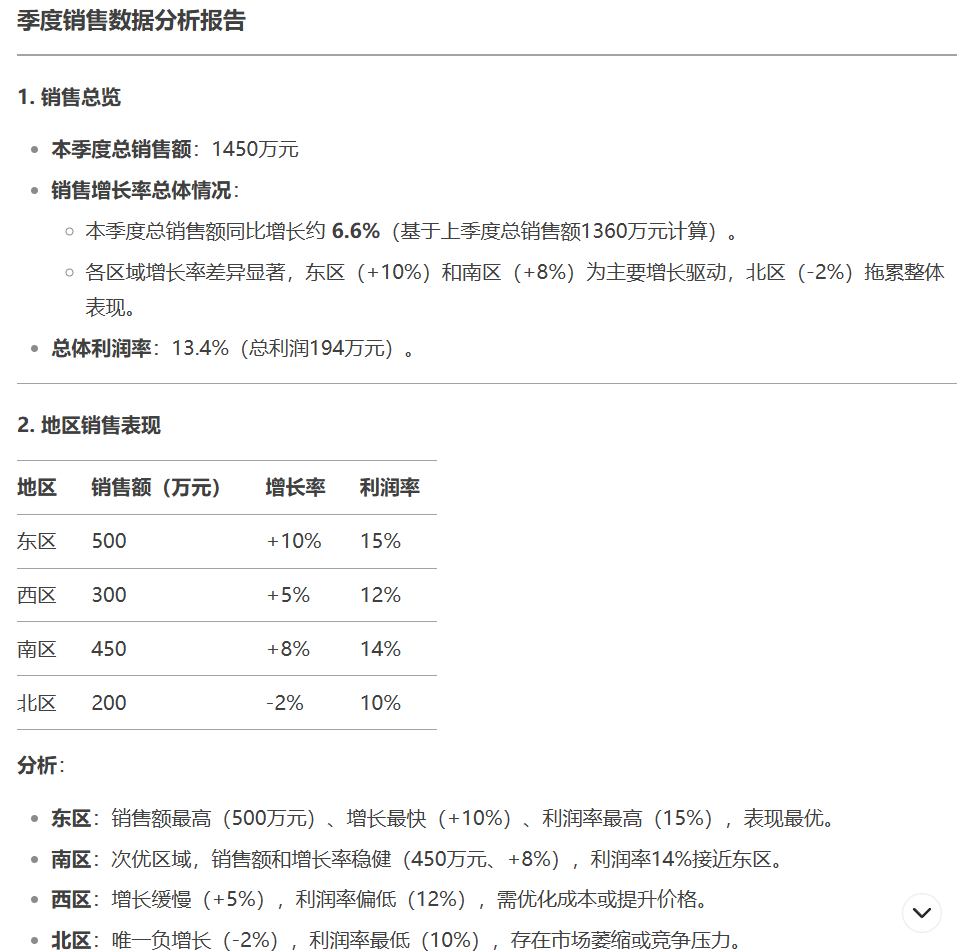
\includegraphics[width=\linewidth]{image/4/生成报告.png}
  \caption{用人工智能助手生成一份报告}
\end{figure}

\subparagraph{4. 后期编辑与优化}

生成的报告内容虽已较为完整,但仍需进行后期编辑和优化,以确保报告的准确性、逻辑性和专业性。具体而言,首先应进行校对和修正,仔细检查生成内容中的语法错误、数据一致性和逻辑连贯性,确保每一处细节都准确无误,使报告内容经得起推敲。其次,要增强报告的专业性,结合企业的具体情况,深入挖掘并补充行业术语和专业分析,让报告在专业领域内更具权威性和说服力,能够精准地传达出企业销售数据背后的深层含义和行业趋势。最后,还需根据实际需求灵活调整报告结构,对报告中的各个部分进行审视,如有必要则增减部分内容,或对章节顺序进行重新排列,使整个报告的结构更加合理、流畅,更好地服务于报告的目的和受众,从而呈现出一份高质量、高价值的企业销售数据分析报告。

\subparagraph{5. 整合可视化元素}

可视化元素在报告中扮演着至关重要的角色,它们不仅能够显著提升报告的可读性,还能增强其说服力,帮助受众更清晰地理解数据背后的信息和趋势。不同类型的图表可以根据数据的特点和报告的需求,选择最合适的方式进行呈现。折线图是展示销售额随时间变化趋势的常见工具,它能够直观地反映出销售业绩的波动和发展趋势,帮助分析者及时发现业务的增长点或瓶颈。饼图则适用于展示不同地区或产品类别的销售占比,通过清晰的比例分布,直观地表达各个部分在整体中的重要性,便于受众快速了解市场结构或资源分配。柱状图则适合用于对比不同地区或产品类别的销售额和利润率,它能够清晰地显示各项数据的相对差异,便于做出具体的业务决策。雷达图则为多维度数据的展示提供了极好的方式,尤其在分析市场竞争力等复杂因素时,雷达图能有效地展示不同维度之间的平衡与差异,使得分析结果更加全面和直观。

为了高效地生成这些图表并将其嵌入报告中,首先需要选择合适的可视化工具。常见的工具如Microsoft Excel、Tableau和Power BI等,各有不同的功能和优缺点,因此应根据企业的实际需求和使用习惯选择最适合的工具。接下来,需要将整理好的销售数据导入到选定的可视化工具中,确保数据的准确性和完整性。根据报告的内容,选择相应的图表类型,并生成对应的可视化图表。此时,生成的图表只是一个初步的草图,为了使其更加美观和易于理解,需要对图表进行进一步的美化,包括调整颜色、字体和布局等,使其不仅具备信息传达功能,还具备视觉吸引力和易读性。最后,将完成的图表嵌入到报告的相应部分,通过图文结合的方式,增强报告的直观性和可读性,帮助读者快速抓住重点,从而提升报告的整体效果和说服力。

\subparagraph{6. 质量校验与最终呈现}

在完成报告内容生成并整合了可视化元素后,下一步是进行全面的质量校验,确保报告的整体质量达到预期标准。质量校验是一个至关重要的环节,它不仅有助于确保报告内容的准确性,还能提升报告的专业性和可读性,从而增强报告的实际效果和影响力。

首先,确保内容的准确性是质量校验中的核心任务。所有数据和分析结果都必须准确无误,任何小小的错误或逻辑漏洞都可能影响报告的可信度和说服力。因此,需对报告中的每一项数据进行严格核查,确保其来源可靠,计算过程无误,分析结论合理。其次,报告的格式规范性也需要仔细检查。这不仅涉及到标题格式、段落结构的统一性,还包括图表布局的合理性。报告的格式必须符合企业的标准,确保各部分内容的排版清晰、整齐,便于阅读。与此同时,报告的逻辑连贯性也非常重要。各部分内容需要紧密相连,层次分明,确保思路清晰,易于读者理解。逻辑不严密或者跳跃性大的报告会让读者产生困惑,进而影响报告的整体效果。

此外,报告的专业性和可读性是衡量报告质量的另一个重要标准。报告语言应保持专业,表达应简明清晰,避免使用过于复杂的术语和冗长的句子。过于晦涩的语言可能会让非专业的读者难以理解,降低报告的可读性。因此,保持平衡,确保报告既能体现专业性,又不失简洁易懂,才是高质量报告的标准。

最后,在所有校验工作完成后,需将校验后的报告导出为PDF或其他适当的格式,进行分发和展示。在此过程中,必须确保报告在不同设备和平台上的兼容性,以便各部门和决策者能够方便地查阅和使用报告的内容。这不仅能提升报告的传播效果,还能确保各方能够迅速获取并依据报告做出决策。

通过上述校验步骤,可以确保报告内容的准确性、逻辑性和专业性,最终呈现出一份高质量、高价值的企业销售数据分析报告,帮助企业做出更精准的决策,推动业务增长。

\paragraph{4. 优化提示设计的技巧}

为了最大化人工智能在报告生成中的效能,需遵循以下提示设计优化技巧:

\begin{enumerate}
    \item \textbf{明确任务目标}:明确描述报告的目的和预期效果,帮助AI准确把握生成内容的方向。
    
    \begin{lstlisting}[language={python},label={},caption={}, basicstyle=\footnotesize\ttfamily, breaklines=true, numbers=left, frame=single]
请生成一份针对本季度销售数据的分析报告,旨在评估各地区和产品类别的销售表现,并提出改进策略。
\end{lstlisting}
    
    \item \textbf{结构化提示}:按照报告的章节和内容进行分步提示,确保AI生成的内容符合预期的结构。
    
    \begin{lstlisting}[language={python},label={},caption={}, basicstyle=\footnotesize\ttfamily, breaklines=true, numbers=left, frame=single]
1. 销售总览
2. 地区销售表现
3. 产品类别分析
4. 市场趋势分析
5. 策略建议
\end{lstlisting}
    
    \item \textbf{提供具体数据和背景信息}:在提示中包含详细的数据表格和相关背景信息,帮助AI进行准确分析。
    
    \begin{lstlisting}[language={python},label={},caption={}, basicstyle=\footnotesize\ttfamily, breaklines=true, numbers=left, frame=single]
以下是本季度的销售数据:

| 地区 | 产品类别 | 销售额(万元) | 销售增长率(\%) | 利润率(\%) |
|------|----------|----------------|------------------|--------------|
| 东区 | A类      | 500            | 10               | 15           |
| 西区 | B类      | 300            | 5                | 12           |
| 南区 | A类      | 450            | 8                | 14           |
| 北区 | C类      | 200            | -2               | 10           |
\end{lstlisting}
    
    \item \textbf{分步引导}:将复杂任务分解为多个小步骤,引导AI逐步生成内容,提升准确性和深度。
    
    \begin{lstlisting}[language={python},label={},caption={}, basicstyle=\footnotesize\ttfamily, breaklines=true, numbers=left, frame=single]
第一步,生成销售总览部分,包括总销售额、销售增长率和总体利润率。

第二步,生成地区销售表现部分,分析各地区的销售额、增长率和利润率。

依此类推,逐步生成报告各部分内容。
\end{lstlisting}
    
    \item \textbf{强调重点和细节}:在提示中突出需要重点分析的部分,确保AI关注关键内容。
    
    \begin{lstlisting}[language={python},label={},caption={}, basicstyle=\footnotesize\ttfamily, breaklines=true, numbers=left, frame=single]
在市场趋势分析部分,重点讨论数字化转型和个性化需求对销售的影响。
\end{lstlisting}
    
    \item \textbf{使用示例和范本}:提供示例格式或范本,帮助AI理解期望的输出形式和风格。
    
    \begin{lstlisting}[language={python},label={},caption={}, basicstyle=\footnotesize\ttfamily, breaklines=true, numbers=left, frame=single]
以下是销售总览部分的示例:

本季度,公司实现总销售额达到1,450万元,较上一季度增长5\%。整体销售增长率为5\%,显示出稳定的增长态势。总体利润率为12.75\%,较上一季度有所提升,表明公司在成本控制和销售策略上取得了一定成效。
\end{lstlisting}
\end{enumerate}

\paragraph{5. 实践中的注意事项}

在实际操作过程中,利用人工智能生成报告时需要注意一些关键点,以确保报告的质量和实用性。首先,数据的准确性与完整性至关重要。确保输入的数据准确无误是避免报告分析失真的前提。此外,数据应全面覆盖报告所需的各个维度,避免遗漏任何重要信息,这样才能确保生成的报告全面且有用。

其次,定期校验AI生成内容的准确性和逻辑性是不可忽视的。若发现问题,应及时进行人工调整,确保AI正确理解提示的意图,避免生成偏离主题的内容。这种做法有助于保证报告的主题和内容始终一致。与此同时,在处理敏感数据时,必须遵循数据隐私保护规范,确保数据安全。使用加密和访问控制措施,防止数据泄露,是保护隐私的必要手段。

为了提升AI生成内容的质量,持续优化提示是一个不可或缺的过程。根据生成报告的质量和反馈,不断调整提示设计,有助于提高报告的相关性和深度。同时,记录有效的提示模板并形成标准化的提示库,能够显著提升生成效率。报告中还应融合行业专业知识和企业实际情况,这不仅增强了报告的专业性,也增加了其实用性。结合AI生成内容与专业人员的见解,可以形成更为全面和有深度的分析报告。

在生成过程中,进行多次迭代也是非常重要的。通过对同一部分内容的多次生成,可以选择最佳版本或综合多个版本的优点,从而提升内容的质量。同时,利用AI的多样性,能够从不同视角分析问题,丰富报告的内涵。对于报告中的视觉元素,也需要确保风格的一致性,以增强整体美观性和专业性。高质量的图表和图片不仅能够提升报告的视觉吸引力,也能使报告更具说服力。

最后,用户反馈在报告生成和优化过程中起着重要作用。收集报告使用者的反馈,了解报告的实用性和可读性,有助于指导后续的优化工作。根据这些反馈及时调整提示设计和报告结构,能够进一步提升报告的针对性和效果。

\subsection{用人工智能快速制作一张插画}

在当今视觉内容需求日益增长的时代,插画作为传达信息、增强视觉吸引力和表达创意的重要手段,广泛应用于广告、出版、网页设计、教育等多个领域。传统的插画创作过程通常需要专业的艺术技能、较长的时间投入以及较高的成本。然而,随着人工智能技术的快速发展,利用 AI 工具快速制作高质量的插画已成为可能。以下将以具体步骤和示例,详细介绍如何通过人工智能快速制作一张插画。

\subsubsection{1.利用人工智能制作插画的步骤}

利用人工智能快速制作插画可以分为如下几个关键步骤:

\textbf{明确需求。} 首先要确定插画需求,包括插画的用途、主题与内容、风格与色彩,以及尺寸与分辨率。例如,某教育机构需要为其新出版的科学教材制作封面插画,主题为“宇宙探索”,风格要求科幻且充满未来感,色彩以蓝色和紫色为主。

\textbf{设计有效的提示词。} 设计详细的提示词(Prompt)是引导 AI 生成符合需求插画的关键。提示词需要包含足够的细节,以确保生成结果与预期一致。这包括描述主题、指定风格、细化元素、色彩要求以及构图布局。例如,可以使用如下提示词:

\begin{lstlisting}[language={python}, label={}, caption={}, basicstyle=\footnotesize\ttfamily, breaklines=true, numbers=left, frame=single]
生成一幅科幻风格的宇宙探索插画,
画面中央是一艘未来感十足的太空飞船,
正在穿越星际。飞船周围有闪烁的星星和遥远的星云,
背景为深邃的宇宙蓝色和紫色调。
飞船设计流线型,表面有闪耀的灯光和复杂的机械结构。
画面整体充满未来科技感,色彩鲜明,细节丰富,
适合作为科学教材的封面插画。
\end{lstlisting}

\textbf{选择 AI 插画生成工具。} 选择合适的 AI 插画生成工具也是至关重要的一步。目前市场上有多种 AI 插画生成工具,如由 OpenAI 开发的 DALL·E、基于 Discord 平台的 Midjourney、开源的 Stable Diffusion 以及 Adobe 推出的 Firefly 等。选择工具时应考虑生成质量、灵活性、易用性和成本等因素。例如,DALL·E 能够根据文本描述生成高质量的图像,而 Stable Diffusion 则具有高度的灵活性,适合个性化定制。

生成初步插画时,将设计好的提示词输入选定的 AI 插画生成工具,生成初步插画。根据工具的不同,可能需要调整提示词或多次尝试以获得理想的结果。例如,在 DALL·E 平台上,可以将提示词粘贴到输入框中,点击“生成”按钮,等待 AI 生成插画,并从多张生成的插画中选择最符合需求的一张。

\textbf{编辑与优化。} 生成的初步插画通常需要进行一定的编辑和优化,以达到更高的视觉效果和使用标准。常见的后期编辑步骤包括颜色调整、细节修饰、背景处理以及添加文本等。例如,对生成的宇宙探索插画进行颜色调整,使蓝色和紫色更具层次感,同时增强飞船的灯光效果,增加星云的细腻度,最终形成一幅高质量的封面插画。

\textbf{整合到应用场景。} 完成插画的编辑和优化后,需要将其整合到所需的应用场景中,如教材封面、网页设计或广告宣传等。例如,可以将优化后的宇宙探索插画作为科学教材的封面,配以标题和副标题,确保封面整体美观且信息传达清晰;在教育机构的官方网站上使用插画作为横幅图片,提升网页的视觉吸引力;或在社交媒体和在线广告中使用插画,吸引潜在用户的关注。

\textbf{质量校验。} 最后,在插画完成后,进行全面的质量校验,确保其符合初始需求和应用标准。质量校验步骤包括视觉审查、内容匹配、风格一致性检查以及收集用户反馈。例如,检查插画的整体视觉效果和细节表现,确认插画是否准确传达了预期的主题和信息,确保插画风格与整体项目或品牌的视觉风格一致,并通过收集使用者或目标受众的反馈,了解插画的接受度和改进建议。根据质量校验和用户反馈,进一步优化插画,或在必要时重新生成插画,以达到最佳效果。

\subsubsection{2.具体示例与操作}

以下通过具体示例,展示如何使用人工智能快速制作一张插画。

\paragraph{示例情境:制作智能家居宣传插画}

某科技公司计划为其最新发布的“智能家居”产品系列制作一张宣传插画,主题定为“未来智能生活”。他们希望插画呈现出现代感和科技感,色调以蓝色和银色为主,以体现产品的高端与未来感。

\textbf{1. 确定插画需求}

插画将用于产品宣传资料、社交媒体推广和官方网站的横幅展示。插画需要展现一个未来智能家居环境,包含智能音箱、智能灯光控制系统和智能安防设备等场景。场景设计应体现现代科技感,突出智能化的生活方式。风格偏向现代科技,色调以蓝色和银色为主,渲染出清爽、高端的科技感。整体效果需具备未来感,带有明显的数字化和智能化元素。插画尺寸要求为横屏宽幅,分辨率不低于 1920$\times$1080 像素,以确保图像在高清设备上展示清晰。

\textbf{2. 设计详细的提示词}

为了最大化地利用人工智能生成插画的潜力,设计了一份清晰且详细的提示词:
\begin{lstlisting}[language={python}, label={}, caption={}, basicstyle=\footnotesize\ttfamily, breaklines=true, numbers=left, frame=single]
请生成一幅现代科技风格的智能家居插画,
画面展示一个未来感十足的客厅,
配备智能音箱、智能灯光系统和智能安防设备。
客厅内的家具设计简洁现代,色彩主要为蓝色和银色,
体现科技感与高端感。墙壁上应有智能显示屏,
显示家庭信息和控制界面。整体氛围明亮、整洁且充满未来感,
适合作为智能家居产品的宣传插画。
\end{lstlisting}

\textbf{3. 选择合适的 AI 插画生成工具}

选择一款可以生成高质量、支持风多样、支持格式丰富的AI作为生成工具

\textbf{4. 生成初步插画}

在使用AI进行插画创作时,进入专门的插画生成界面。在平台的文本框中,输入已经设计好的详细提示词,这些提示词将指导 AI 模型生成符合需求的插画。稍作等待后,AI 模型会根据输入的提示词生成几幅插画,用户可以浏览这些插画并选择最符合项目需求的一张作为最终作品。如果初次生成的插画效果未能完全达到预期,用户可以通过调整提示词中的细节,优化描述,从而更精确地引导 AI 生成符合设计要求的插画,并再次进行生成。通过这种方法,用户能够不断微调提示词,直到获得理想的插画效果。

\textbf{5. 后期编辑与优化}

在生成初步插画后,接下来的步骤是使用图片编辑软件对插画进行进一步的编辑和优化,以提升其视觉效果。首先,通过颜色调整,增强蓝色和银色的饱和度,使得插画中的色彩更加鲜明,层次感更强,进而突显出未来感和科技感。接下来,细节增强是优化的关键之一,尤其是智能设备的外观设计。在这一环节中,可以加入光线反射效果、微妙的阴影和光晕,进一步加强设备的立体感,并营造出更加深邃的科技氛围。最后,在插画的上方添加“未来智能生活”字样,使用简洁现代的字体,确保文字的颜色与整体色调和风格协调搭配,这样既能突出主题,又不会破坏插画的整体视觉美感。通过这些细致的编辑,插画的科技感和未来感将得到更好的呈现,同时也增强了其作为宣传工具的吸引力和视觉冲击力。

\textbf{6. 整合与应用}

将最终优化后的插画整合到科技公司的官方网站横幅和产品宣传资料中,确保插画与其他设计元素(如文字、按钮、布局)协调一致。通过精心的排版和设计,使插画不仅提升视觉效果,还能够更好地吸引用户的注意力,传递品牌的智能、创新形象。

\textbf{7. 质量校验与反馈}

在插画的应用阶段,进行严格的质量校验是至关重要的一步,以确保最终作品符合设计要求并能够有效传达宣传主题。首先,进行视觉审查,检查插画的色彩是否鲜明,细节是否清晰,以避免出现模糊或失真的现象。其次,进行内容匹配的审查,确保插画中展示的智能家居环境和智能设备元素准确反映了宣传主题,能够有效地传达产品的核心价值和特点。风格一致性同样不可忽视,检查插画的风格是否与公司品牌的整体视觉形象保持一致,确保品牌识别度并提升品牌形象的统一性。最后,将插画展示给目标用户群体,收集他们的反馈意见,并根据用户的建议进行必要的优化和调整。通过这一过程,进一步提高插画的接受度和效果,确保插画不仅符合公司要求,还能够引起目标受众的共鸣,从而增强宣传效果。

通过上述步骤,成功制作出一幅充满现代感和未来感的智能家居插画。AI 生成插画不仅大大缩短了设计制作时间,还降低了成本,同时保证了插画的高质量和专业性。最终的插画作品完美符合科技公司宣传需求,成为吸引潜在客户的视觉亮点,充分展示了人工智能技术在创作和设计领域的巨大潜力和高效性。

\subsubsection{3.优化提示技巧的应用}

在实际操作中,设计高效的提示对于生成符合需求的插画至关重要。通过合理地编写和优化提示词,可以帮助 AI 更加精准地理解并呈现设计需求。以下是一些经过实践验证的提示优化技巧,能在较大程度上提高插画生成的质量和准确度。

\textbf{明确描述需求。} 在提示词中详细描述插画的主题、风格、色彩以及需要呈现的具体元素。避免使用模糊或含糊的词汇,以免 AI 产生不符合预期的结果。

\begin{lstlisting}[language={python}, label={}, caption={}, basicstyle=\footnotesize\ttfamily, breaklines=true, numbers=left, frame=single]
生成一幅现代科技风格的智能家居插画,
画面展示一个未来感十足的客厅,
配备智能音箱、智能灯光系统和智能安防设备……
\end{lstlisting}

\textbf{使用具体的关键词。} 在提示词中加入明确且具体的关键词,可以使 AI 更准确地理解目标场景或效果。

\textbf{分步骤描述。} 将插画的整体布局和细节要求分解成若干步骤,一条条地写明。这样能让 AI 逐项生成,并在每一条指令下对特定元素进行精细化处理,避免遗漏或混淆。

\textbf{提供参考示例。} 如果有心仪的风格或相似主题的插画,可将其作为参考示例,让 AI 更直观地了解目标效果,从而生成更贴合设计期望的插画。

\textbf{迭代优化。} 完成初次生成后,如果插画效果与预期存在差距,可根据具体问题对提示词进行针对性调整,反复迭代。每次微调提示词都能让 AI 朝更理想的成品方向前进。

通过应用以上五个技巧,用户可以更好地引导人工智能模型,生成符合预期且高质量的插画作品。在此过程中,不仅能够显著提升插画生成的准确度,也进一步展现了人工智能在创意设计领域的巨大潜力。

\subsubsection{4.小结}

通过具体案例的展示,可以清晰地看到提示工程在实际应用中的强大功能。以企业销售数据分析报告和插画制作为例,借助人工智能不仅能够大幅提高内容生成的效率,还能确保输出的高质量和专业性。关键在于如何设计高效的提示,明确任务需求,提供具体的数据和细节,并通过后期编辑和优化,充分发挥人工智能模型的潜力。在未来,随着人工智能技术的不断进步和提示工程的不断优化,其在各类实际应用中的价值将进一步凸显,助力各行业实现智能化转型和高效运营。

\section{总结}

本章深入探讨了提示工程这一人工智能的新兴领域,从了解提示工程开始,向读者介绍提示工程的定义,发展历程等,使其对提示工程有了简单的认识。然后,详细介绍多种提示技巧,包括基于样本数量、基于思考过程、基于一致性和连贯性等,并且附上相应的例子,形象直观地引领读者接触并使用这些技巧。最后,从实际应用出发,详细介绍提示工程的应用,让读者对提示工程的使用有一个更加清楚的认识。

\section{习题}
\begin{enumerate}
\item \textbf{提示工程的内涵包括哪些?}

(1)对人工智能模型工作原理的深入理解

(2)融合了跨学科的知识与技能

\item \textbf{提示工程和提示词的区别是什么?}

(1)提示词是用户与模型交互的具体文本输入,是提示工程的直接产物。

(2)提示工程是人工智能领域的一个新兴领域,针对人工智能模型设计和构建特定的提示,以引导模型按照预期的方式生成内容、执行任务或做出决策。

\item \textbf{简要概述提示工程的重要性。}

(1)提升模型性能

(2)拓展应用边界

(3)增强人机协作

(4)推动技术创新

\item \textbf{如何设计一个好的提示?}

(1)明确任务目标,即明确传达出希望模型完成的具体任务

(2)提供足够的背景信息,使模型理解任务的背景和要求

(3)使用清晰的语言并可以结合自身需求提供简单例子

\item \textbf{基于样本数量的提示词技术和基于思考过程的提示词技术的适用范围有什么区别?}

(1)基于思考过程的提示词技术通过引导模型逐步进行推理,模拟人类的思考过程,适用于需要多步推理和逻辑分析的任务。

(2)基于样本的提示词技术(如少样本提示)通过提供少量示例,帮助模型快速理解任务的模式和规则,适用于模式识别任务。

\item \textbf{简述如何用人工智能快速制作一张插画?}

(1)确定自身对插画的需求

(2)设计详细描述需求的提示词

(3)选择合适的生成工具并进行插画的初步生成

(4)结合自身需求进行后续编辑和优化

\item \textbf{思考一下当前提示工程有哪些不足之处?}

(1)提示可能因为描述等方面出现歧义,难以生成预期的结果

(2)模型自身性能的限制

(3)难以处理多模态融合的提示

(4)伦理问题

\item \textbf{提示工程的实际应用有哪些?}

(1)自然语言处理任务:问答系统、文本生成、翻译、情感分析等。

(2)代码生成与编程辅助:生成代码片段、优化编程任务。

(3)复杂任务分解:将复杂任务分解为多个子任务逐步完成。

(4)多模态任务:结合图像、音频等多模态数据提升协同工作效率。

(5)行业应用:报告生成、图片插画生成等。

\item \textbf{提示工程未来可能有哪些发展方向?}

(1)多模态的提示工程,即将文本、图像、音频等多种数据格式结合在一起。

(2)自动化提示工具的发展,可以根据AI的输出动态调整提示,生成更加符合需求的答案,以减少人工迭代的需要。
\end{enumerate}